% !TEX root = thesis.tex

%\section{Introduction}
%
%\begin{abstract}
%
%\end{abstract}
\tableofcontents
%\listoffigures

\clearpage
\section{Introduction}
\label{sec:introduction}
This thesis focuses on studying Quantum Chromodynamics (QCD)~\cite{gross1973asymptotically}, a part of the standard model of particle physics~\cite{Tanabashi:2018oca}, which is the theory describing the strong interactions. Strong interaction is the force responsible for interactions that holds the nucleus of an atom together. Fundamentally it describes the interactions between quarks and gluons, the elementary constituents of the building blocks of the nucleus, protons and neutrons. Because of specifics of this interaction quarks and gluons, together dubbed partons, can never be seen free~\cite{Perl:2004qc}. Under ordinary conditions they are confined into bound states called hadrons. In extreme conditions they can form a medium of asymptotically free quarks and gluons, guark-gluon plasma (QGP)~\cite{Shuryak:1980}. %Understanding QGP is the holy grail of heavy-ion physics

Indirectly quarks can be seen in high energy particle collisions as jets, collimated streams of particles observed in high energy particle collisions~\cite{Perkins:1982xb}. The physics of these jets is the primary topic discussed in this thesis. Understanding jets is important when one is interested in the processes that produce the partons that eventually fragment into jets. By themselves jets can provide an insight into QCD when the fragmentation is studied. Jets can also be used as probes of the QGP medium. 

Experimentally jets are often studied with a jet reconstruction algorithm which clusters observed tracks to find a reasonable estimate of the initial parton. That is also the case in this thesis. The main observable studied is the jet fragmentation transverse momentum \jt{} which is defined as the perpendicular component of the momentum of jet constituents with respect to the jet axis, the best estimate of the initial parton. As such \jt{} measures the transverse nudge that fragmentation products receive.

The analysis studies collisions between protons and lead nuclei. Originally these were meant to be a reference for lead-lead collisions to rule out possible cold nuclear matter effects~\cite{Connors:2017ptx}; effects caused by the regular 'cold' nuclear matter of a nucleus as opposed to QGP. However, \pPb collisions have provided interesting physics by themselves. Many of the collective phenomena that in \PbPb collisions were attributed to QGP have been observed also in high multiplicity \pPb collisions~\cite{Nagle:2018nvi} and even in ultra high multiplicity \pp collisions~\cite{Nagle:2018nvi}. However observables of jet modification show no conclusive signals in \pPb collisions~\cite{Connors:2017ptx,Nagle:2018nvi}. %So far all observables have focused on 

This thesis is organised as follows: Section ~\ref{sec:introduction} first gives a general introduction into the history and properties of QCD and heavy-ion physics. It is followed by a description of hard processes, jet fragmentation and hadronisation and how these processes might look like in a heavy-ion environment. Finally there is a discussion on the physics of small systems.

The experimental setup that was used to collect the data in this thesis is described in Section ~\ref{sec:exp}. It starts by explaining the accelerator facilities at CERN and LHC in more detail. This is followed by a description of the ALICE experiment and its sub-detectors. A part of Section ~\ref{sec:exp} is dedicated to coming upgrades of ALICE as this is a timely topic. In 2019-2020 ALICE will be upgraded and I have made a personal contribution to the TPC upgrade.

Section ~\ref{sec:selection} gives a description of the event, track and cluster selection criteria used in the analysis. This is followed in Section ~\ref{sec:methods} by the specific analysis methods used in this thesis. First the jet reconstruction algorithm used, anti-\kt{}, is described. Section ~\ref{sec:methods} continues by introducing the \jt{} observable, how it is obtained and what methods are used to estimate background contribution and correct for detector effects. Finally the fitting method used for the final results is described. Section 5 gives the different systematic uncertainties that arise from the analysis.

Finally the results from the analysis are presented in Section ~\ref{sec:results}. The results are compared to \pythia~and Herwig Monte Carlo generators. Further discussion of the results is given in Section~\ref{sec:disc} when the results are compared to \jt{} results obtained with a different analysis method. Section~\ref{sec:sum} summarises the main results and gives an outlook for future.


\pagebreak
\subsection{Quantum chromodynamics}
\subsubsection{Foundation of QCD}
The universe is governed by four basic interactions: gravity, electromagnetic, weak and strong interactions. The standard model of particle physics~\cite{Tanabashi:2018oca} includes three of these, electromagnetic, weak and strong interactions.  The fourth one, gravity, is described well in all but the most extreme of cases by the theory of general relativity~\cite{Einstein1915}. The standard model is a quantum field theory where local gauge symmetries dictate  particle interactions~\cite{Perkins:1982xb}. 

The first interaction included in the standard model was the electromagnetic interaction. The foundations of quantum field theory and Quantum Electrodynamics (QED) were already laid out by the work by Dirac in 1927~\cite{doi:10.1098/rspa.1927.0039}. The full theory of QED was formulated in 1946-1949 by Tomonaga~\cite{Tomonaga:1946zz},  Schwinger~\cite{Schwinger:1948yj,Schwinger:1948yk} and Feynman~\cite{Feynman:1948fi}% and Dyson~\cite{Dyson:1949bp},
%for which they received the Nobel prize in physics in ~\

Motivated by the success of a quantum field theory approach for the electromagnetic interaction physicists started working on the remaining interactions. However, the weak and strong nuclear interactions proved more challenging to formulate~\cite{Krauss:2017}. In the end the weak interaction was unified with the electromagnetic interaction into the electroweak theory. The final theory was formulated by Glashow~\cite{Glashow:1970gm}, Salam~\cite{Salam:1964ry} and Weinberg~\cite{Weinberg:1967tq}.

The theory of strong interactions became to be known as Quantum Chromodynamics (QCD). The search for a theory of strong interactions began after the formulation of QED and drew further inspiration when new powerful particle accelerators capable of particle physics research were introduced in the 1950s. Before this the main source of particle physics was the study of cosmic rays. From cosmic ray studies positrons, neutrons and muons were discovered in the 1930s and charged pions were discovered in 1947~\cite{Occhialini:1987nr,Lattes:1947mx}. The neutral pion was discovered in 1950~\cite{Bjorklund:1950}.

The Lawrence Berkeley National Laboratory started the Bevalac accelerator in 1954, Super Proton Synchrotron (SPS) in CERN began operating in 1959 and the Alternating Gradient Synchrotron (AGS) at Brookhaven started in 1960. AGS  was the most powerful accelerator of that time with an energy of \unit[33]{\gev}. By the beginning of 1960s several new particles had been discovered. These included antiprotons~\cite{Chamberlain:1955ns}, antineutrons~\cite{Cork:1957nu}, $\Delta$-particles and the six hyperons ($\Xi^0$\cite{Alvarez:1959zz}, $\Xi^-$~\cite{Armenteros:1952nt}, $\Sigma^{\pm}$~\cite{Bonetti1953}, $\Sigma^0$~\cite{Plano1957} and $\Lambda$~\cite{Fowler:1953qpk}).

Facing this avalanche of new particles, physicists started the search for symmetries within them. Already in 1932 Heisenberg~\cite{Heisenberg:1932} 
had proposed an isospin model to explain similarities between the proton and the neutron. In 1962 Gell-Mann and Ne'eman showed that particles sharing the same quantum numbers (spin, parity) could be organised using the symmetry of SU(3)~\cite{Gell-Mann:1962}. Heisenberg's Isospin model had followed the symmetry of SU(2). Using the SU(3) model known baryons and mesons could be presented as octets. This lead to the discovery of the $\Omega^{-}$~\cite{Barnes:1964ga} particle as the SU(3) decouplet that included heavier baryons was missing a baryon. 

The most simple representation of SU(3) is a triplet. Inside this triplet particles would have electric charges $\nicefrac{2}{3}$ or $-\nicefrac{1}{3}$. However, particles like these had not been detected. In 1964 Gell-Mann~\cite{Gell-Mann:1964} and Zweig~\cite{Zweig:1964jf} proposed that baryons and mesons would be bound states of these three hypothetical triplet particles that Gell-Mann called quarks and Zweig called aces. Now we know that these are the $u$, $d$ and $s$ quarks. However, this original quark model without colour still had a problem as it was violating the Pauli exclusion principle. For example the $\Omega^{-}$ particle is comprised of three $s$ quarks, two of which would have exactly the same quantum states, since spin can only have two values. 


Greenberg had already presented the idea of colour in 1964~\cite{Greenberg:1964}. In 1971 Gell-Mann and Fritzsch presented their model~\cite{Fritzsch:1972jv}, which added a colour quantum number to quarks. This separated quarks of the same species solving the antisymmetry problem. In the new colour model the baryonic wave function became

\begin{equation}
\left( qqq\right)\rightarrow\left(q_rq_gq_b-q_gq_rq_b+q_bq_rq_g-q_rq_bq_g+q_gq_bq_r-q_bq_gq_r\right),
\end{equation}


%improve
\noindent The colour model was also supported by experimental evidence like the decay rate of a neutral pion. When taking colour into account the decay rate is

\begin{equation}
\Lambda\left(\pi^0\rightarrow\gamma \gamma\right) = \frac{\alpha^2}{2\pi}\frac{N_c^2}{3^2}\frac{m_\pi^3}{f_\pi^2}.
\end{equation} 

\noindent For $N_c=3$ this gives \unit[7.75]{eV} while the measured value is $(7.86\pm0.54)\,\mathrm{eV}$~\cite{Williams:1988sg}.

Another observable combining the colour information to the number of quark flavours is the Drell-Ratio $R$~\cite{Krolikowski:1974jx}

\begin{equation}
R=\frac{\sigma\left(e^++e^-\rightarrow\mathrm{hadrons}\right)}{\sigma\left(e^++e^-\rightarrow\mu^++\mu^-\right)}=N_c\sum_fQ_f^2.
\end{equation}

\noindent This ratio has the numerical value 2 when the three light quarks $u$, $d$ and $s$ are included. When the collision energy reaches the threshold of heavy quark ($c$ and $b$) production processes this increases to $\nicefrac{10}{3}$ (for $f=u,d,s,c$) and \nicefrac{11}{3} (for $f=u,d,s,c,b$). The energy threshold ($\sqrt{s}\approx\unit[350]{\gev}$) of $t\bar t$ production, has not been reached so far by any $e^+e^-$ colliders.

%\cite{Glashow:1970gm} Introduction of lepton-quark symmetry by Glashow,Iliopoulos and Maiani, proposal of a fourth (charmed) quark.
%\\cite{Bacci:1974za} ADONE Discovery of charm quark and $J/\Psi$
%\cite{Aubert:1974js} BNL
%\cite{Augustin:1974xw} SLAC


In the colour model only colour neutral states are possible which explains why no free quarks had been observed. The simplest ways of producing a colour neutral object are baryons, the combination of three quarks, and mesons, the combination of a quark-antiquark pair. Although the hunt for more exotic combinations has been going on for decades, only in 2019 did LHCb produce conclusive evidence of the observation of a pentaquark~\cite{Aaij:2019vzc}, a state which consists of 4 quarks and one antiquark.

First experimental indication of the existence of quarks came in 1969 when a series of experiments at the Stanford Linear Accelerator Center (SLAC) revealed that protons and neutrons appeared to have some substructure~\cite{Bloom:1969kc, Breidenbach:1969kd}. For this discovery they eventually received the Nobel Prize in Physics in 1990~\cite{Nobel1990}. Bjorken demonstrated that these results could be explained if protons and neutrons were composed of virtually noninteracting pointlike particles~\cite{Bjorken:1968dy,Bjorken:1969ja}. Feynman~\cite{Feynman:1969ej} interpreted these objects as real particles and suggested they would be the quarks of Gell-Mann's model. At the time, however, this seemed mysterious; if all strongly interacting particles, hadrons, were composed of quarks, then quarks should surely be strongly interacting themselves. Why would they appear to be almost free inside hadrons? This turned out to be a key clue in formulating the theory of strong interactions~\cite{Krauss:2017}.

After the addition of colour the main ingredients of QCD had been established and the final quantum field theory of Quantum Chromodynamics formed quickly between 1972 and 1974. Main part of this was the work by Gross, Wilczek, Politzer and George for non-abelian gauge field theories~\cite{gross1973ultraviolet, politzer1973reliable, gross1973asymptotically, gross1974asymptotically, georgi1974electroproduction}. The work showed that quarks would indeed be asymptotically free in a non-abelian theory, which explained the results from SLAC. Gross, Wilczek and Politzer received the Nobel Prize in Physics for their work~\cite{Nobel2004}. The role of gluons as a colour octet mediating the strong interaction was presented by Fritzsch, Gell-Mann and Leutwyler in 1973~\cite{fritzsch1973advantages}. %The theory had now 8 massless gluons to mediate the strong interaction.

%Nobel1990 to Friedman, Kendall and Taylor for SLAC results
%Nobel1976 to Richter and Ting

The quark model was extended in 1974 when the discovery of the charm quark and the first charmed hadron, $J/\Psi$, was simultaneously published by teams from the SLAC~\cite{Augustin:1974xw}, from Brookhaven National Laboratory~\cite{Aubert:1974js} and from the ADONE collider in Frascati, Italy~\cite{Bacci:1974za}. In 1976 the Nobel Prize in Physics was awarded to Richter and Ting for the discovery of the charm quark~\cite{Nobel1976}. The existence of a fourth quark had already been speculated in 1964 by Bjorken and Glashow~\cite{Bjorken:1964gz}, but a proper prediction was provided by Glashow, Iliopoulos and Maiani in 1970~\cite{Glashow:1970gm} based on symmetries between leptons and quarks in weak interactions.

However, the mediating particles, gluons, had not been discovered. Indirect evidence of the existence had been seen as it was observed that only about half of the momentum of protons was transported by the quarks~\cite{25gluons}. Direct evidence was first seen in 1979 at the PETRA accelerator at DESY~\cite{Brandelik:1979bd, PhysRev.43.830, Berger1979418} in the form of a three jet event, where the third jet came from a gluon.

The two remaining quarks, bottom and top, were introduced by Kobayashi and Maskawa in 1973 to explain CP-violation~\cite{Kobayashi:1973fv}. For this they received the Nobel Prize in Physics in 2008~\cite{Nobel2008}. Bottom quark was discovered soon after, in 1977, at Fermilab~\cite{Herb:1977ek}. The heaviest quark, top quark, would eventually be discovered in 1995 by the CDF~\cite{Abe:1995hr} and DØ~\cite{Abachi:1994td} experiments at Fermilab.




\subsubsection{Asymptotic Freedom}
In Quantum Electrodynamics (QED) the vacuum becomes polarised in the vicinity of a charge. Virtual particle-antiparticle pairs populate the surroundings of the centre charge.
%Virtual particles with opposite charge are attracted, and virtual particles with like charge are repelled by the original charge. 
The net effect is that the field at any finite distance is partially cancelled. Closer to the central charge one sees less of the vacuum effect and the effective charge increases. With increasing distance to the charge the effective charge decreases until the coupling constant of QED reaches the fine-structure constant $\alpha=\frac{1}{137}$~\cite{Perkins:1982xb}.

%The net effect is to partially cancel out the field at any finite distance. Getting closer and closer to the central charge, one sees less and less of the effect of the vacuum, and the effective charge increases.

%In Quantum Electrodynamics (QED) the electric charge is screened. In the vicinity of a charge, the vacuum becomes polarized. Virtual charged particle-antiparticle pairs around the charge are arranged so that opposing charges face each other. Since the pairs also include an equal amount opposite charge compared to the original charge the average charge seen by an observer at a distance is smaller. 


There is screening also in QCD because of the colour charges. However, QCD is a non-abelian theory, i.e. the generators of the symmetry group of QCD, SU(3), do not commute. The practical consequence is that gluons interact also with other gluons while in QED the neutral mediating particles, photons, only interact with charged particles. The self-interaction of gluons leads to the antiscreening of the colour charge which dominates over the screening effect. Thus for larger distances to the central charge the coupling constant is larger. This explains why no free colour charges can be observed. With increasing distance between charges the interaction becomes stronger until it is strong enough to produce a new quark-antiquark pair. On the other hand, at very small distances the coupling constant approaches zero. This is known as asymptotic freedom~\cite{Perkins:1982xb}.

%Contrary to QED, QCD is a non-abelian theory. In other words the generators of the symmetry group of QCD, SU(3), do not commute. This has the practical consequence that gluons interact also with other gluons, whereas in QED the neutral carrier particles, photons, only interact with charged particles.
%There is screening also in QCD because of the colour charges, but in addition to that there is antiscreening because of the gluon interactions. In QCD the antiscreening effect dominates over screening. Thus for larger distances to the colour charge the coupling constant is larger. This explains why no free colour charges can be observed. When the distance between charges increases the interaction strengthens until it is strong enough to produce a new quark-antiquark pair. On the other hand, at very small distances the coupling constant approaches zero. This is called asymptotic freedom~\cite{Perkins:1982xb}.

Based on asymptotic freedom Collins predicted in 1975~\cite{Collins:1975} a state where individual quarks and gluons would no longer be confined into hadronic states. Instead they form a bulk QCD matter that was later coined Quark-Gluon Plasma (QGP) by Edward Shuryak in his 1980 review of QCD and the theory of superdense matter~\cite{Shuryak:1980}. QGP can be seen as a separate phase of hadronic matter and thus a phase diagram can be drawn. Figure~\ref{fig:QCDphase} shows a schematic view of this phase diagram from QCD matter.

\begin{figure}[htb]
\centering
%\includegraphics[width=0.9\textwidth]{pics/qcd_ms_high}
\includegraphics[width=0.9\textwidth]{pics/QCDphase2.pdf}
\caption[QCD phase diagram]{A schematic illustration of the phase diagram of QCD matter at ultra-high density and temperature. The $x$-axis, showing the quark chemical potential $\mu$, represents the imbalance between quarks and antiquarks. Along the $x$-axis the temperature is zero. Along the vertical axis the temperature increases, which takes us through the crossover from a hadronic gas to quark-gluon plasma. With low $\mu$ this is the regime explored by high-energy heavy-ion colliders~\cite{Rajagopal:2001} and also the trajectory taken by the universe when it cooled after the Big Bang. The conditions in neutron stars correspond to the lower right corner, with low $T$ and high $\mu$.}
\label{fig:QCDphase}
\end{figure}


In the early universe at the age of $10^{-6}\mathrm{s}$ after the Big Bang the conditions preferred the existence of QGP instead of hadronic matter. Nowadays QGP, its properties and the phase transitions between it and hadronic matter can be explored in laboratories, through collisions of heavy atomic nuclei at ultra-relativistic energies. The phase transition in QCD is the only phase transition in a quantum field theory that can be probed by current or foreseeable technology. Thus the study of QCD matter at high temperature is of broad interest.

One important property of QGP is the shear viscosity to entropy ratio, $\eta/s$. It is believed that this ratio has an universal minimum value of $1/4\pi \approx 0.08$, among all substances in nature. This limit is reached in the strong coupling limit of certain gauge theories~\cite{Kovtun:2004de}. Figure~\ref{fig:etas} shows the temperature dependance of $\eta/s$ for several substances. For all cases the minimum value of $\eta/s$ is found in the vicinity of the critical temperature, $T_c$~\cite{PhysRevLett.98.092301}. Therefore studying the $\eta/s$ ratio in QGP matter could also probe the critical point of QCD matter.

The $\eta/s$ value for the matter created in Au--Au collisions at RHIC ($\sqrt{s_{NN}}=\unit[200]{\gev}$) has been estimated to be $0.09\pm0.015$~\cite{PhysRevLett.98.092301}, which is very close to the proposed minimum value, suggesting that the matter created does go through a phase where it is close to the critical point of QCD.
% for a wide class of thermal quantum field theories~\cite{Kovtun:2004de} for all relativistic quantum field theories at finite temperature and zero chemical potential. 

\begin{figure}[htb]
\centering
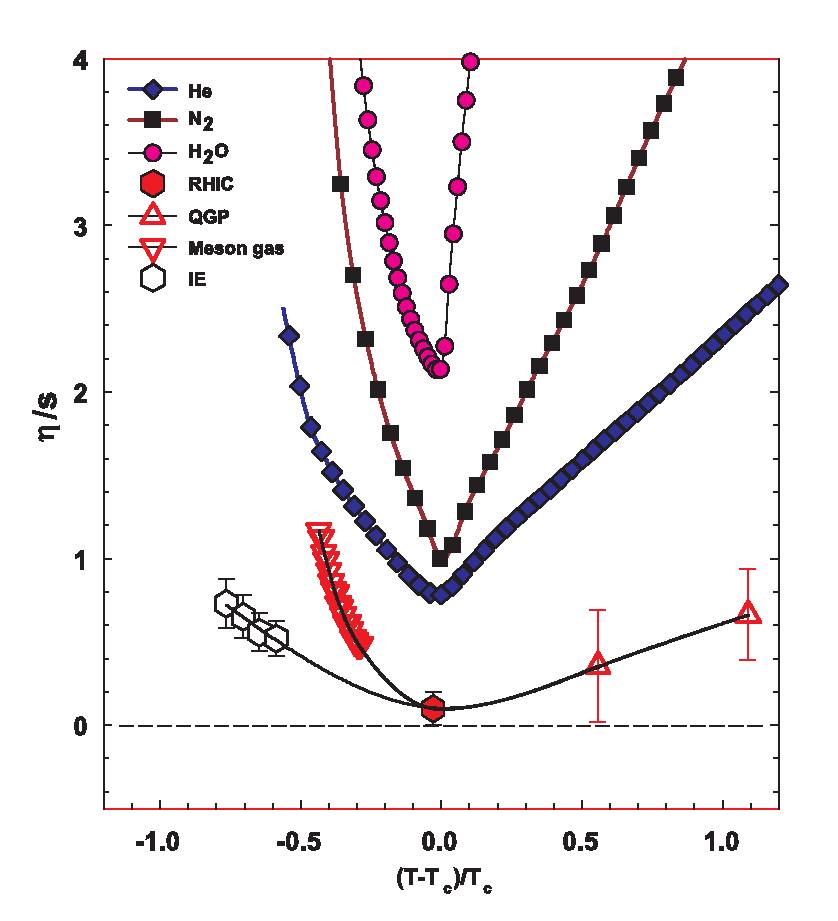
\includegraphics[width=0.9\textwidth]{pics/eta-s-vs-t-tc3}
\caption[$\eta/s$ vs $(T-T_c)/T_c$]{The figure shows \label{fig3}$\eta/s$ as a function of $(T-T_c)/T_c$ for several substances as indicated. The lines are drawn to guide the eye. The $\eta/s=0.09\pm0.015$ value at RHIC is estimated from Au--Au collisions at $\sqrt{s_{NN}}=\unit[200]{\gev}$. The calculated values for the meson-gas have an associated error of $\sim$ 50\%. The calculations assume a value $T_c = \unit[170]{\mev}$ for nuclear matter. ~\cite{PhysRevLett.98.092301}
}
\label{fig:etas}
\end{figure}



\FloatBarrier
\pagebreak
\subsection{Heavy-ion physics}
Quark Gluon Plasma (QGP) can be experimentally studied by colliding heavy-ions at high energies. Nowadays research of heavy-ion collisions is mainly performed at two particle colliders; The Relativistic Heavy-Ion Collider (RHIC) at BNL in New York, USA and the Large Hadron Collider (LHC) at CERN in Switzerland. Energy densities at these colliders are assumed to be large enough to produce QGP and indeed convincing evidence of QGP has been seen at both colliders. Complimentary research with heavy nuclei is also performed at the Super Proton Synchrotron (SPS) at CERN.

%The history of heavy-ion physics is strongly connected to the development of particle colliders. Experimental study of relativistic heavy-ion collisions has been carried out for three decades, beginning with the Bevalac at Lawrence Berkeley National Laboratory (LBNL)~\cite{Lofgren_1975}, and continuing with the AGS at Brookhaven National Laboratory (BNL)~\cite{Barton:1987}, CERN SPS~\cite{Vitev:2002pf}, culminating today with RHIC at BNL and LHC at CERN. 
%
%%The first colliders could not produce enough energy to create QGP matter so they could only probe the hadronic state. 
%%
%%The collective motion of matter in a heavy-ion collision has been modeled using several models e.g. the Blast wave Model~\cite{PhysRevC.84.064905} has been used succesfully. Another model growing in popularity is the hydrodynamical approach which is further discussed in section \ref{sec:hydro}.
%
%\subsubsection{History}
The first heavy-ion collisions were performed in fixed target experiments at the Bevalac experiment at the Lawrence Berkeley National Laboratory~\cite{Lofgren_1975} and at the Joint Institute for Nuclear Research in Dubna~\cite{kovalenko1994status}, which reached energies of up to \unit[1]{\gev}1 per nucleon.
In 1986 the Super Proton Synchrotron (SPS) at CERN started to look for QGP signatures with O--Pb collisions where the centre-of-mass energy per colliding nucleon pair $\left(\sqrt{s_{NN}}\right)$ was \unit[19.4]{\gev}~\cite{Vitev:2002pf}. However, no decisive evidence of QGP was found in these initial experiments. In 1994 a heavier lead (Pb) beam was introduced for new experiments in SPS at $\sqrt{s_{NN}}\approx \unit[17]{\gev}$. Simultaneously the Alternating Gradient Synchrotron (AGS) at BNL started colliding ions up to $\mathrm{^{32}S}$ with a fixed target at energies of up to \unit[28]{\gev}~\cite{Barton:1987}. In 2000 CERN~\cite{SPSpress} presented compelling evidence for the existence of a new state of matter in SPS. Today SPS is used for fixed-target experiments with \unit[400]{\gev} proton beams. One of these is the SPS heavy-ion and Neutrino Experiment (SHINE)~\cite{Grebieszkow:2013nza}, which tries to search for the critical point of strongly interacting matter.

The Relativistic heavy-ion Collider (RHIC) at BNL in New York, USA started its  operation in 2000. The top centre-of-mass energy per nucleon pair at RHIC, \unit[200]{\gev}, was reached in the following years with Au--Au collisions. The results from the experiments at RHIC have provided a lot of convincing evidence that QGP was created~\cite{Adcox:2004mh, Adams:2005dq, Arsene:2004fa, Back:2004je}. The newest addition to the group of heavy-ion accelerators is the Large Hadron Collider (LHC) at CERN, Switzerland. LHC started operating with proton-proton collisions in November 2009. A year later, in November 2010, first \PbPb heavy-ion runs began at $\sqrt{s_{NN}}=2.76\; \mathrm{TeV}$. Since then LHC has provided both \PbPb and \pPb collisions and a short period of Xe--Xe collisions. Table~\ref{tab:datasets} shows a summary of these. Among the main experiments at LHC, the (a) Large Ion Collider Experiment (ALICE) is dedicated to heavy-ion physics. Also CMS and ATLAS have active heavy-ion programs and LHCb uses its SMOG system~\cite{Maurice:2017iom} to perform unique fixed target collisions with heavy ions. 


\begin{table}[htb]
\centering
\caption{Summary of datasets. The integrated luminosities are from ALICE.}
\label{tab:datasets}
\begin{tabular}{| c | S | c |}
\hline
\multicolumn{3}{| c |}{Run 1 (2009-2013)} \\
\hline
\multirow{4}{*}{\pp} & 0.9 \tev & $\sim \unit[200]{\mu b^{-1}}$ \\
 & 2.76 \tev & $\sim \unit[100]{n b^{-1}}$ \\
 & 7.0 \tev & $\sim \unit[1.5]{p b^{-1}}$ \\
 & 8.0 \tev & $\sim \unit[2.5]{p b^{-1}}$ \\
 \hline
\pPb & 5.02 \tev & $\sim\unit[15]{n b^{-1}}$ \\
\hline
\PbPb & 2.76 \tev & $\sim \unit[75]{\mu b^{-1}}$ \\
\hline
\end{tabular}
\begin{tabular}{| c | S | c |}
\hline
\multicolumn{3}{| c |}{Run 2 (2015-2018)} \\
\hline
\multirow{2}{*}{\pp} & 5.02 \tev & $\sim \unit[1.3]{p b^{-1}}$ \\
 & 13.0 \tev & $\sim \unit[25]{p b^{-1}}$ \\
 \hline
\multirow{2}{*}{\pPb} & 5.02 \tev & $\sim\unit[3]{n b^{-1}}$ \\
& 8.16 \tev & $\sim\unit[25]{n b^{-1}}$ \\
\hline
Xe--Xe & 5.44 \tev & $\sim \unit[0.3]{\mu b^{-1}}$ \\
\hline
\PbPb & 5.02 \tev & $\sim \unit[1]{n b^{-1}}$ \\
\hline
\end{tabular}
\end{table}

\pagebreak
\FloatBarrier
%\pagebreak
\subsection{Features of heavy-ion collisions}
\label{sec:features}
\subsubsection{Collision Geometry}
\label{sec:geometry}
In contrast to protons, atomic nuclei have considerable transverse size. This gives a collision between nuclei geometric properties that provide insight into the collision dynamics.  One illustration of a heavy-ion collision is shown in Figure~\ref{fig:planes}. The main defining parameter of a collision is the vector connecting the centres of the two colliding nuclei at their closest approach, which is known as the impact parameter $\vec b$.

The reaction plane is defined by $\vec b$ and the beam direction. The reaction plane angle $\Psi_{RP}$ gives the angle of the reaction plane in the experimental reference frame, which is fixed by the detector setup. Reaction plane angle cannot be directly measured in high energy nuclear collisions, but it can be estimated with the event plane method~\cite{Voloshin:2008dg}. 
\begin{figure}[h!]
\centering
%\definecolor{primary}{HTML}{0000FF}
%\definecolor{secondary}{HTML}{FF8000}
%\definecolor{tertiary}{HTML}{00FFFF}
%\begin{tikzpicture}
%      \draw[->] (-4,0) -- (4,0) node[below] {$x$};
%      \draw[->] (0,-3) -- (0,3) node[left] {$y$};
%       \coordinate[] (C);
% \coordinate[left=1cm of C] (C1);
%\coordinate[right=1cm of C] (C2);
%\draw[dashed, thick, primary] (C1) circle (2cm);
%\draw[dashed, thick, secondary] (C2) circle (2cm);
%      
%\end{tikzpicture}

\includegraphics[width=0.6\textwidth]{pics/Definitions}
\caption[The definitions of the Reaction Plane coordinate systems]{The definition of the Reaction Plane coordinate systems~\cite{Voloshin:2007pc}. The dashed circles represent the two colliding nuclei and the green dots are partons that take part in the collision. $x_{RP}$ is the reaction plane.} %The angle between $x_{RP}$ and $x_{PP}$ is given by Eq. (\ref{eq:partangle}). $y_{PP}$ and $y_{RP}$ are lines perpendicular to the participant and reaction planes. }
\label{fig:planes}
\end{figure}


The length of the impact parameter is one way to quantise the centrality of a heavy-ion collision but it is not possible to measure $\vec b$ in a collision. Any estimation from observed data must use theoretical models and is thus model-dependent. To compare results between different experiments one needs a general definition for centrality. %The difference between central and peripheral collisions is illustrated in Figure~\ref{fig:collisionA}. In a central collision the overlap region is larger than in a peripheral collision. Larger overlap region translates into a larger number of nucleons participating in the collision, which in turn leads to a larger number of particles produced in the event.





%\begin{figure}[h!]
%\centering
%        \begin{subfigure}[b]{0.45\textwidth}
%                \centering
%            	\includegraphics[height=1in]{pics/Collisionperipheral}
%                \caption{Peripheral collision}
%                \label{fig:peripheral}
%        \end{subfigure}
%        \begin{subfigure}[b]{0.45\textwidth}
%                \centering
%               \includegraphics[height=1in]{pics/Collisioncentral}
%                \caption{Central collision}
%                \label{fig:central}
%        \end{subfigure}
%        \caption[Interaction between partons in central and peripheral collisions.]{Interaction between partons in central and peripheral collisions. The snowflakes represent elementary parton-parton collisions. When the impact parameter $b$ is large the number of elementary collisions is small. Particle production is small. Smaller impact parameter increases the number of elementary collisions. This increases  particle production.}\label{fig:collisionA}
%\end{figure}

Instead of the impact parameter, in practice centrality is defined by dividing events into percentile bins by the number participants or by the observed multiplicity. Small centrality percentages correspond to central events with the highest multiplicity and high centrality percentages correspond to more peripheral collisions with lower multiplicities. Figure~\ref{fig:centrality} shows an observed multiplicity distribution from ALICE measurements~\cite{PhysRevC.88.044909} with the centrality bin division. The distribution is fitted using a phenomenological approach that combines a Glauber Monte Carlo calculation~\cite{Miller:2007ri} and the convolution of a model for the particle production and a negative binomial distribution. 


\begin{figure}[tb]
\centering

               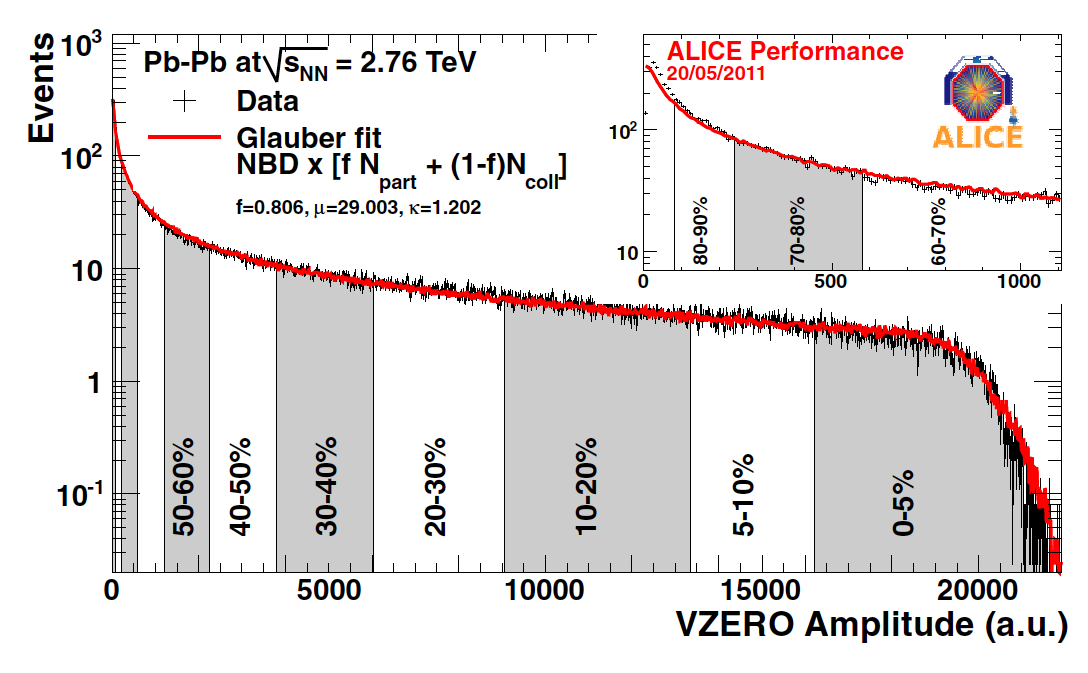
\includegraphics[width=0.9\textwidth]{pics/centrality.png}
        \caption[An illustration of the multiplicity distribution in ALICE measurement with centrality classes.]{An illustration of the multiplicity distribution which is divided into centrality bins in ALICE measurements~\cite{PhysRevC.88.044909}. The red line shows the fit of the Glauber calculation to the measurement.}
        	\label{fig:centrality}
\end{figure}


The Glauber Model is often used to model the nuclear geometry in a heavy-ion collision. The model was originally introduced already in 1958~\cite{Glauber:1959} and the modern terminology and tools were introduced in 1976~\cite{Biallas1976461} by Białłas, Bleszyński, and Czyż to model inelastic nuclear collisions.


The model starts by defining the thickness function which is the integral of the nuclear density over a line going through the nucleus with minimum distance $s$ from its centre

\begin{equation}
T_A\left(s\right)=\int_{-\infty}^{\infty}\dd z \rho\left(\sqrt{s^2+z^2}\right),
\end{equation}

\noindent where $ \rho\left(\sqrt{s^2+z^2}\right)$ is the number density of nuclear matter. This can be experimentally determined by studying the nuclear charge distribution in low-energy electron-nucleus scattering experiments~\cite{Miller:2007ri,DeJager:1987qc}. For a spherically symmetric nucleus a good approximation is given by the Woods-Saxon potential~\cite{Abelev:2013qoq}

\begin{equation}
\rho\left( r\right) = \frac{\rho_0 \left(1+\omega r^2 / R^2\right)}{1+\exp \left(\frac{r-R}{a}\right)},
\end{equation}


\noindent where $\rho_0$ is the nucleon density in the centre of the nucleus, $R$ is the nuclear radius, $a$ parametrizes the depth of the skin and $\omega$ can be used to introduce a surface excess. Figure~\ref{fig:woodssaxon} shows how this distribution looks like with parameters observed for lead nuclei. With $\omega=0$ the density stays relatively constant as a function of $r$ until it drops to almost 0 around $R$. The slope and length of the transition region is given by $a$. 

\begin{figure}
\centering
\begin{tikzpicture}
      \draw[->] (0,0) -- (7,0) node[below] {$r\left[\unit{fm}\right]$};
      \draw[->] (0,0) -- (0,5) node[left] {$\nicefrac{\rho}{\rho_0}$};
      \draw	(0,0) node[anchor=north] {0}
		(3,0) node[anchor=north] {5}
		(6,0) node[anchor=north] {10};

      \draw	(0,2) node[anchor=east] {0.5}
		(0,4) node[anchor=east] {1};
	
      \draw[dashed,black] (3.8,0) -- (3.8,5);

	
     \draw[black,thin,<->] (0,2) -- node[above] {$R$} (3.8,2);
     \draw[black,thin,<->] (3.55,1) -- node[below] {$a$} (4.05,1);
     
     \draw[blue] (2,3.5) node {$\omega=0$};
     \draw[blue] (2,4.5) node {$\omega>0$};

      \draw[scale=0.6,domain=0:10,smooth,variable=\x,blue,dashed] plot ({\x},{(6.66+1*\x^2/6.38^2)/(1+exp((\x-6.38)/0.546))});
       \draw[scale=0.6,domain=0:10,smooth,variable=\x,blue] plot ({\x},{(6.66)/(1+exp((\x-6.38)/0.546))});

      %\draw[scale=0.5,domain=-3:3,smooth,variable=\y,red]  plot ({\y*\y},{\y});

\end{tikzpicture}
\caption{Woods-saxon distribution, with typical values for a Pb nucleus, $a=0.55\unit{fm}$ and $R=6.6\unit{fm}$.}
\label{fig:woodssaxon}
\end{figure}


The integral over the overlap area of two thickness functions of colliding nuclei defines the overlap function. This can be seen as the material that takes part in the collision. It is given as a function of the impact parameter $b$

\begin{equation}
T_{AB}\left(\vec b\right)=\int \dd{^2s} T_A\left(\vec s\right) T_B\left(\vec s - \vec b\right)
\end{equation}

\noindent The average overlap function, $\left<T_{AA}\right>$, in an A-A collisions  is given by~\cite{Afanasiev:2009aa}

\begin{equation}
\left<T_{AA}\right>=\frac{\int T_{AA}\left(b\right) \dd b}
{\int\left(1-e^{-\sigma^{inel}_{pp}T_{AA}\left(b\right)}\right)\dd b}.
\end{equation}

\noindent Using $\left<T_{AA}\right>$ one can calculate the mean number of binary collisions

\begin{equation}
\left<N_{coll}\right>=\sigma_{pp}^{inel}\left<T_{AA}\right>,
\end{equation}

\noindent where the total inelastic cross-section, $\sigma_{pp}^{inel}$, gives the probability of two individual nucleons interacting. As each binary collision has equal probability for direct production of high-momentum partons the number of high momentum particles is proportional to $\left<N_{coll}\right>$~\cite{Abelev:2013qoq,Kharzeev:2004if,Deng:2010mv}. This requires knowledge of $\sigma\mathrm{^{NN}_{inel}}$, which can be measured in proton-proton collisions at different energies. At the LHC the most precise cross section measurements come from TOTEM~\cite{Antchev:2017dia}.

On the other hand, soft production is based on the number of participants~\cite{Kharzeev:2004if}. It is assumed that in the binary interactions participating nucleons get excited and further interactions are not affected by previous interactions since the time scales are too short for any reaction to happen in the nucleons. After the interactions excited nucleons produce a predictable number of soft particles. The average number of participants, $\left<N_{part}\right>$ can be calculated from the Glauber model 


\begin{eqnarray}
\left<N_{part}^{AB}\left(\vec b\right)\right>&=&\int \dd{^2s} T_A\left(\vec s\right)\left[1-\left[1-\sigma_{NN}\frac{T_B\left(\vec s - \vec b\right)}{B}\right]^B\right] \nonumber \\
 &+ &\int \dd{^2 s} T_B\left(\vec s\right)\left[1-\left[1-\sigma_{NN}\frac{T_A\left(\vec s - \vec b\right)}{A}\right]^A\right].
\end{eqnarray}



There are two common approaches to Glauber calculations. The optical approximation is one way to get simple analytical expressions for the nucleus-nucleus interaction cross-section, the number of interacting  nucleons and the number of nucleon-nucleon collisions on average. In the optical Glauber it is assumed that  the nucleons move independently during the crossing of the nuclei and they will be essentially undeflected.  

With increased appreciation for the physics emerging from fluctuations in the collision geometry the Glauber Monte Carlo (GMC) approach has emerged as a method to get a more realistic description of the collisions. In GMC nucleons are distributed randomly according to the nuclear density distribution~\cite{Abelev:2013qoq}. In the simplest model nucleons of two nuclei will interact if their distance in the orthogonal plane, $d$ is small enough, i.e. 

%A heavy-ion collision is then treated as a series of independent nucleon-nucleon collisions, where in the simplest model nucleons interact if their distance  in the plane orthogonal to the beam axis, $d$, satisfies

\begin{equation}
d< \sqrt{\sigma\mathrm{^{NN}_{inel}}}.
\end{equation}

\noindent The average number of participants and binary collisions can then be calculated and by simulating many nucleus-nucleus collisions one can determine both average values and the fluctuation around the average. The results of one GMC \PbPb event with impact parameter $b=\unit[9.8]{fm}$ is shown in Figure~\ref{fig:GMC}.

\begin{figure}[htbp]
\centering
               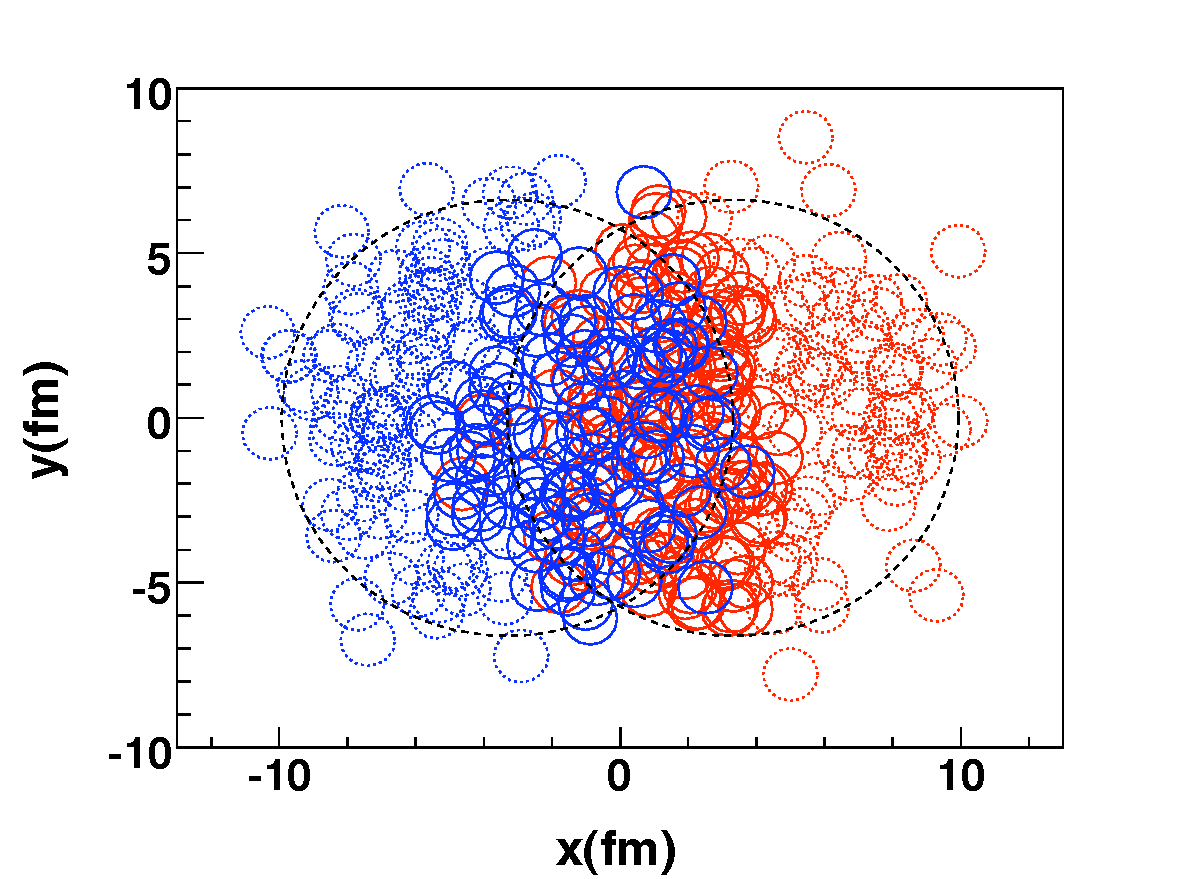
\includegraphics[width=0.75\textwidth]{figures/test_pbpb_2a}
        \caption[The result of one Glauber Monte Carlo simulation.]{The figure shows one Glauber Monte Carlo simulation for a \PbPb collision. Big circles with black dotted boundaries represent the two colliding nuclei. Small red and blue circles represent nucleons with different colours for the nuclei. Circles with solid boundaries are participants i.e. they interact with at least one nucleon from the other nucleus. Circles with dotted boundaries are spectators which do not take part in the collision~\cite{Alver:2008aq}.}
        	\label{fig:GMC}
\end{figure}



\subsubsection{Collective motion}
\label{sec:collective}
For most cases the evolution of a heavy-ion event can be divided into four stages. A schematic representation of the evolution of the collisions with this division is shown in Figure~\ref{fig:HISpaceTime}. Stage 1 is the phase immediately after the collision. This is known as the pre-equilibrium stage. It is commonly assumed to last about $1\ \mathrm{fm}/c$ in proper time $\tau$. 
%Hydrodynamic description is not applicable to this regime because thermal equilibrium is not yet reached. 

\begin{figure}[htb]
\centering
               \includegraphics[width=0.75\textwidth]{pics/HISpaceTime2}
        \caption[Schematic representation of a heavy-ion collision]{Schematic representation~\cite{Romatschke:2009im} of a heavy-ion collision as a function of time and the longitudinal coordinate $z$. The various stages of the evolution are separated by hyperbolic curves which are defined by fixed proper time $\tau=\sqrt{t^2-z^2}$.}
        	\label{fig:HISpaceTime}
\end{figure}

Thermal equilibrium or at least a near-equilibrium is reached during the second stage. This lasts about $5-10\ \mathrm{fm}/c$ until the temperature of the system sinks low enough for the system to lose its deconfined, strongly coupled state and hadronisation occurs. During this stage the matter begins to expand as it is driven outwards by the large pressure difference between the centre of the collision and the vacuum outside the collision volume.

During stage 3 the hadrons still interact with each other. This ends when hadron scattering becomes rare and they no longer interact. In the final stage hadrons are free streaming and they fly in straight lines until they reach the detector. 

In a heavy-ion collision the bulk collective particle production that is emitted from the QGP medium is referred to as flow. During hadronisation the pressure-driven expansion of QGP is transformed into the flow of low-momentum particles. Since the expansion is close to isotropic the resulting particle flow is isotropic with small anisotropies of the order of $10\%$ at most. The isotropic part of flow is referred to as radial flow. 

%In this stage hydrodynamics should be applicable if the temperature is above the deconfinement temperature~\cite{Romatschke:2009im}. 
% strongly coupled, state and hydrodynamics can no longer be used.






\begin{figure}[b!]
\centering
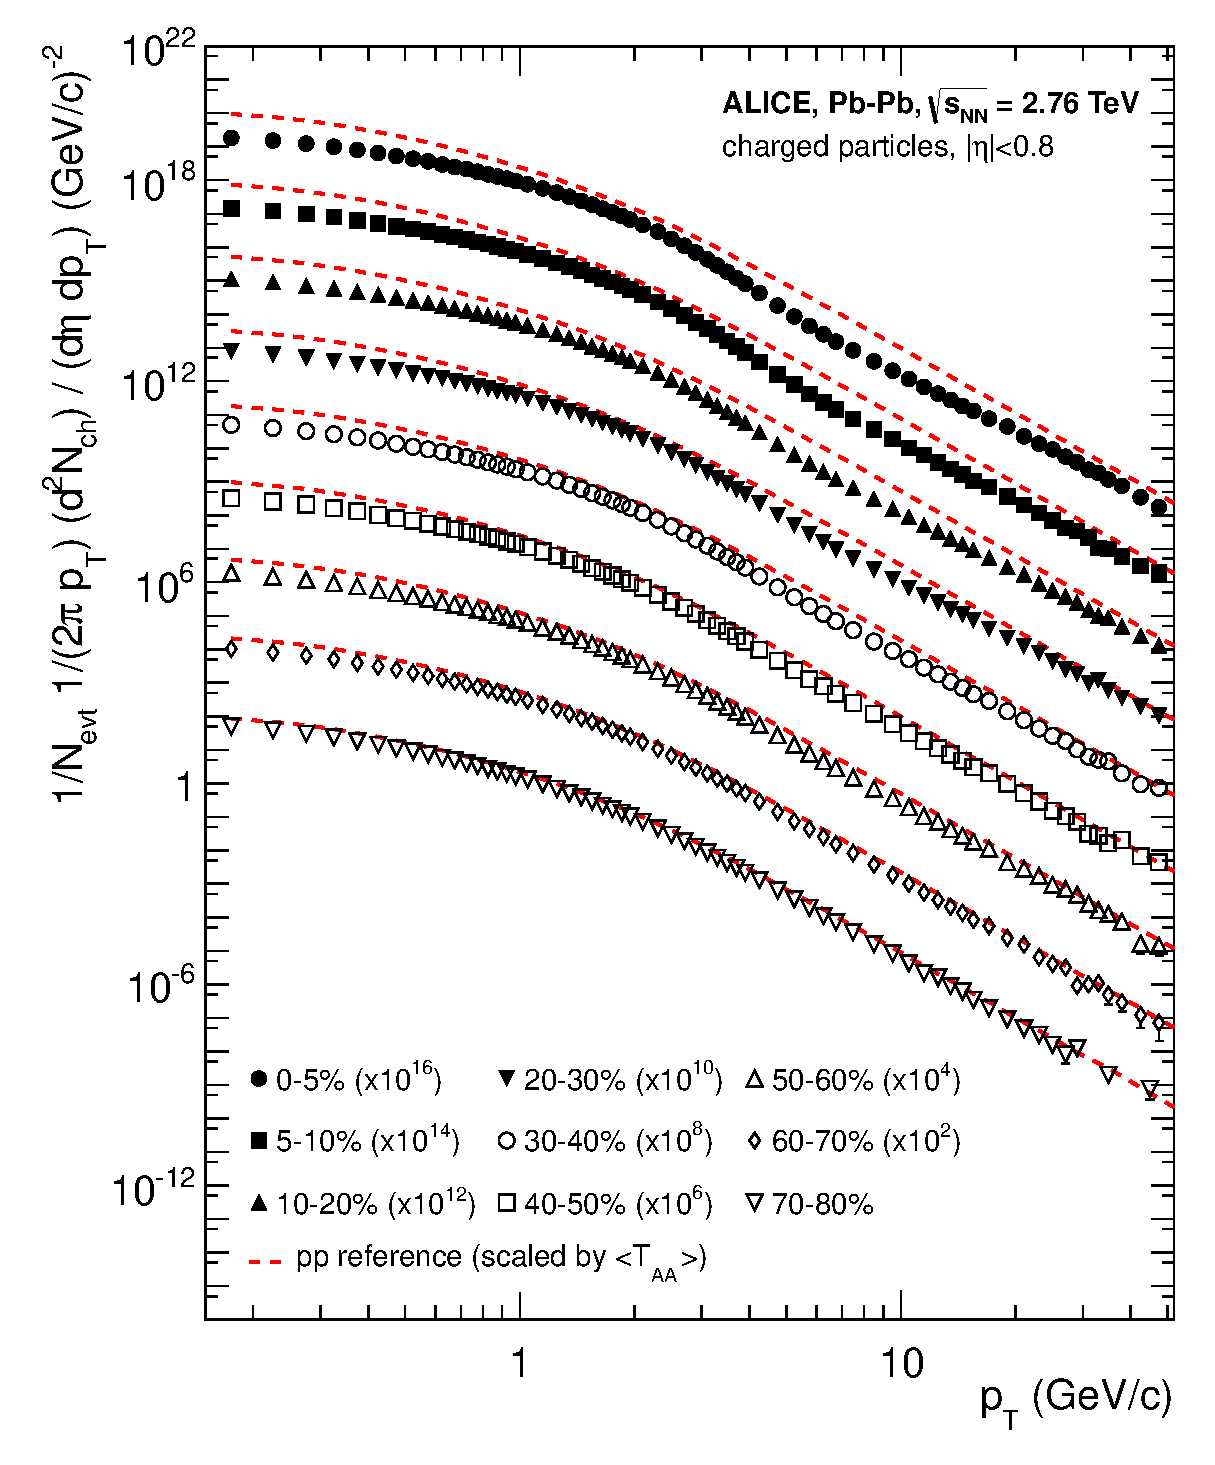
\includegraphics[width=0.6\textwidth]{pics/pT_PbPb}
\caption[Charged particle spectra]{ Charged particle spectra measured by ALICE~\cite{PRL106032301} for the 9 centrality classes given in the legend. The dashed lines show  proton-proton reference spectra which are scaled by the nuclear overlap function determined for each centrality class~\cite{PRL106032301}.  For clarity the distributions and the reference spectra are offset by arbitrary factors.}
\label{fig:dndpt}
\end{figure}

Figure~\ref{fig:dndpt} shows the transverse momentum spectra $\dd N/\dd {\pt{}}$ in heavy-ion collisions. As the vast majority of produced particles have small $\pt{}$, any observables that are integrated over $\pt{}$ are dominated by the small momentum region of the spectrum. The difference between the yield of $\unit[1]{\gevc}$ and $\unit[4]{\gevc}$ particles is already 2-3 orders of magnitude.

The geometry of the heavy-ion collision produces an anisotropic component to the collective motion. Figure~\ref{fig:flow} gives illustrations of collisions with different impact parameters. In a non-central heavy-ion collision, with a large impact parameter, the shape of the impact zone is almond-like. In a central collision, with a small impact parameter, the overlap region is almost circular in the transverse plane.

\begin{figure}[b!]
\centering
        \begin{subfigure}[b]{0.52\textwidth}
                \centering
            	%\includegraphics[height=2.4in]{pics/InteractionB}
	         \includegraphics[height=2.4in]{figures/tikz/central}

                \caption{Peripheral collision}
                \label{fig:InteractionB}
        \end{subfigure}
        \begin{subfigure}[b]{0.45\textwidth}
                \centering
              % \includegraphics[height=2.4in]{pics/InteractionA}
                \includegraphics[height=2.4in]{figures/tikz/peripheral}

                \caption{Central collision}
                \label{fig:InteractionA}
        \end{subfigure}
	\caption[Illustration of flow in momentum space in central and peripheral collisions.]{Illustration of flow in central and peripheral collisions. The density of the arrows represent the magnitude of flow in the corresponding azimuthal direction at a large distance from the collision. In a peripheral collision momentum the difference in pressure gradients gives a strong flow into the in-plane direction while the flow into the out-of-plane direction is weak. In a central collision anisotropy in flow is smaller. In the figure the difference is exaggerated and the difference in total multiplicity is not taken into account.}
	\label{fig:flow}
\end{figure}

The pressure gradient is largest in-plane, in the direction of the impact parameter $\vec b$, where the distance from high pressure, at the collision centre, to low pressure, outside the overlap zone, is smallest. This produces stronger collective flow along the direction of $\vec b$, which in turn results in enhanced thermal emission through a larger effective temperature into this direction, as compared to the out-of-plane direction~\cite{Ollitrault:1992,Ollitrault:1993, Heinz:2002}. The resulting flow is illustrated in Figure~\ref{fig:flow}. %Flow with two maxima in the direction of the reaction plane is called elliptic flow. 

Flow anisotropy is typically quantified in the form of a Fourier composition 

\begin{equation}
E\frac{\dd{^3N}}{\dd {p^3}}=\frac{1}{2\pi}\frac{\dd {^2N}}{\pt{ }\dd {\pt{ }}\dd {\eta} } \left(1+\sum_{n=1}^{\infty}2v_n\left(\pt{},\eta\right)\cos(n(\phi-\Psi_n))\right),
%\label{eq:finalseries}
\end{equation}

\noindent where the coefficients $v_n$ give the relative contributions of different flow components and the overall normalisation, $\frac{1}{2\pi}\frac{\dd {^2N}}{\pt{ }\dd {\pt{ }}\dd {\eta} }$, gives the strength of radial flow. Elliptic flow, i.e. flow with two maxima, is represented by $v_2$ and $v_3$ represents triangular flow. The first coefficient, $v_1$, is connected to directed flow~\cite{Voloshin:1994mz}. This is in total assumed to be zero because of momentum conservation. In certain rapidity or momentum regions it can be nonzero but it must be canceled by other regions.

In a peripheral collision $v_2$ is the dominant part of anisotropic flow as it arises from the asymmetric geometry of the collision region.  For a long time it was believed that the odd harmonics would be negligible. In 2007 Mishra {\emph et al.}~\cite{Mishra:2007tw} argued that density inhomogeneities in the initial state would lead to non-zero $v_n$ values for higher harmonics including $v_3$. Higher harmonics come from fluctuations in the initial conditions~\cite{Alver:2010gr}. As the colliding nuclei are not static objects, the arrangement of the nucleons at the time of a collision is random. Therefore the shape of the collision zone is not symmetric. Instead it can have a more complex shape. Also inside the collision zone the density of the created medium is not homogenous but it can have hot spots with higher density. It is expected that higher harmonics of $v_n$ would be suppressed more by viscous effects and that the shape of $v_n$ as a function of $n$ would provide another valuable tool for studying $\eta/s$~\cite{Mocsy:2010um}.

The first one to predict anisotropic flow in heavy-ion collisions was Ollitrault in 1992~\cite{Ollitrault:1992}. However, the first papers on anisotropy did not use the Fourier composition. Instead they approached the problem with a classic event shape analysis. The first experimental studies of anisotropy were performed at the AGS~\cite{PhysRevLett.70.1393} in 1993, where it was noted that the anisotropy of particle production in one rapidity region correlates with the reaction plane angle defined in another rapidity region. The first ones to introduce the Fourier decomposition were Voloshin and Zhang in 1996~\cite{Voloshin:1994mz}.

\begin{figure}[tb]
	\centering
	\begin{subfigure}[t]{0.5\textwidth}
                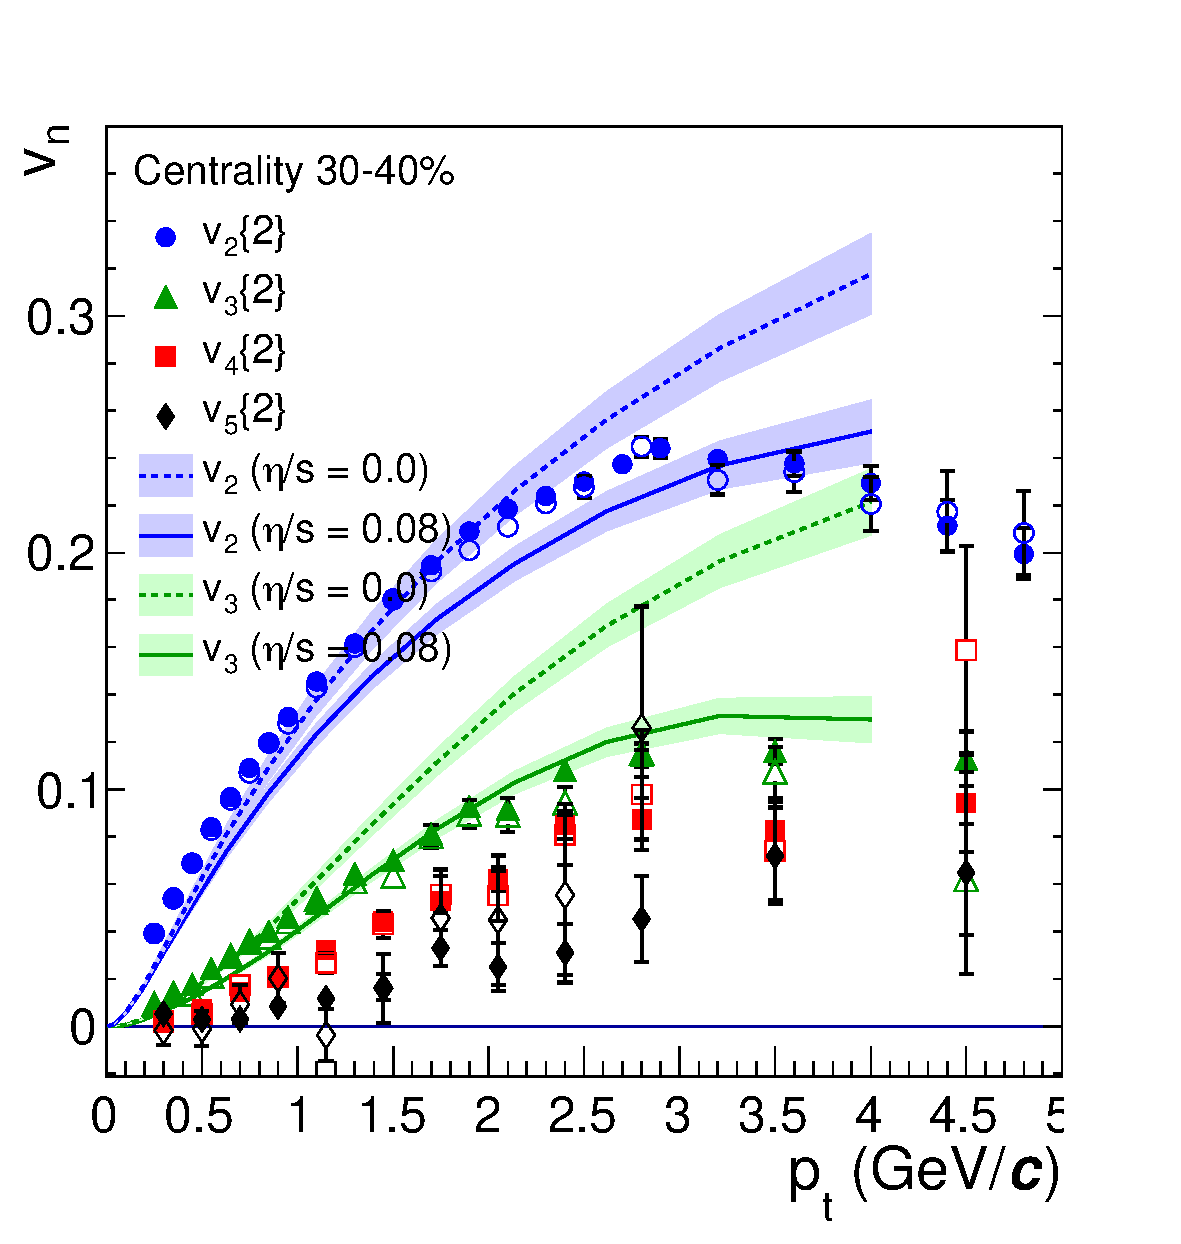
\includegraphics[width=\textwidth]{pics/alice_vn_figa.pdf}
        %\caption[ALICE measurement of $v_2$, $v_3$, $v_4$, $v_5$]{ALICE measurement of $v_2$, $v_3$, $v_4$, $v_5$ as a function of transverse momentum. The flow coefficients are determined by two-particle correlations using different rapidity separations.  The full and open symbols are for $\Delta\eta > 0.2$ and $\Delta\eta > 1.0$. The results are compared to hydrodynamic predictions~\cite{Schenke:2011tv} with different values of $\eta/s$~\cite{PRL107032301}.}
        \label{fig:higherharmonics}
        \end{subfigure}
        \quad
        \begin{subfigure}[t]{0.45\textwidth}
        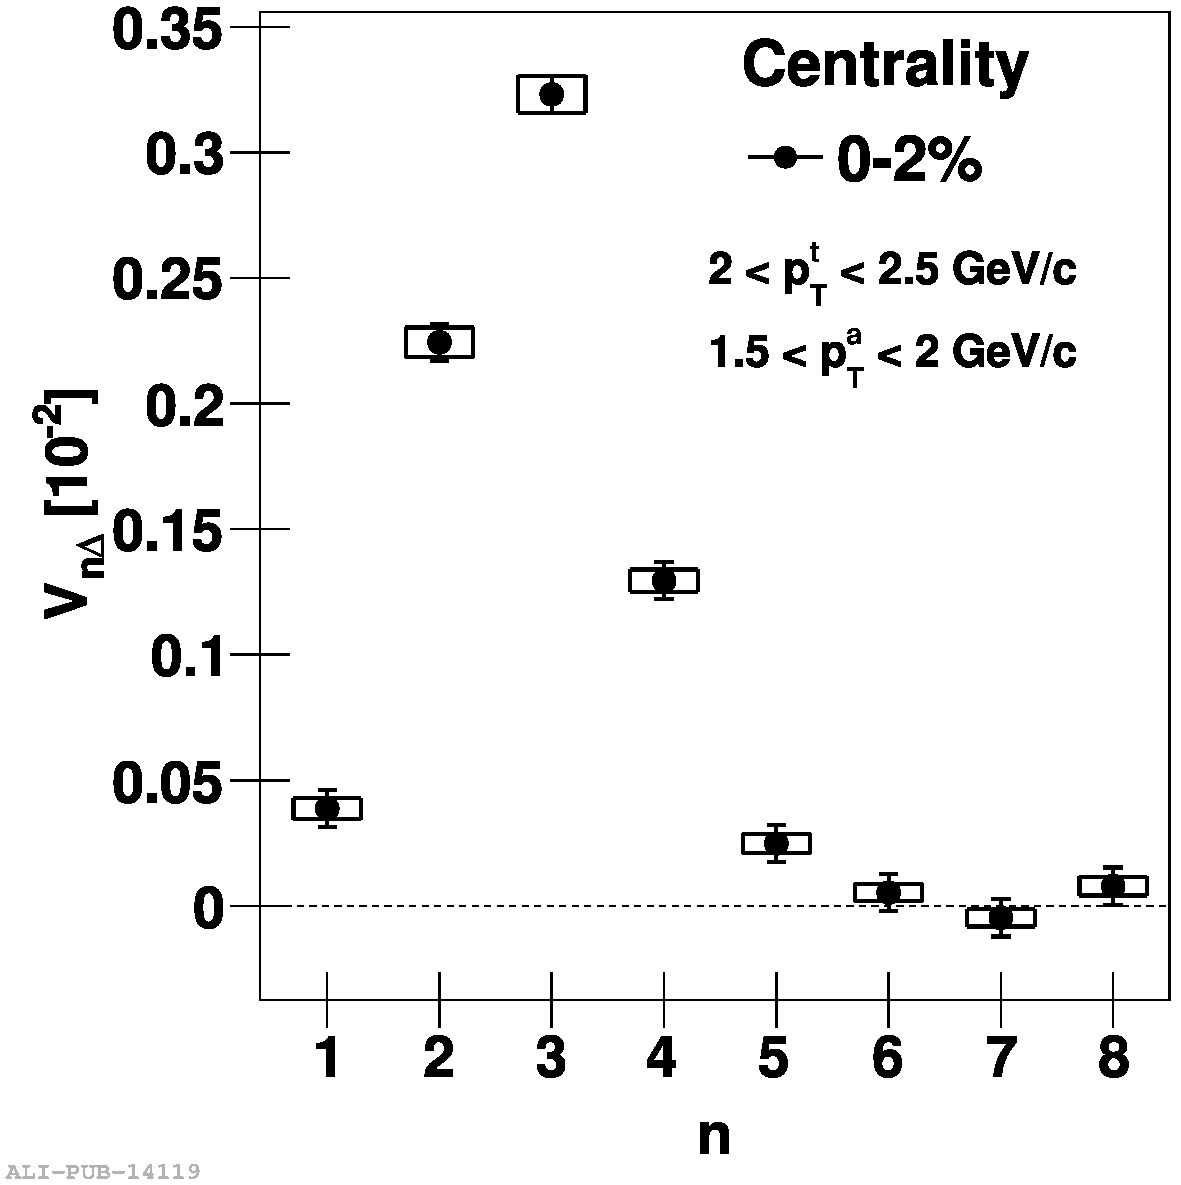
\includegraphics[width=\textwidth]{pics/2012-Jun-06-fig02b}
       % \caption{Amplitude of $v_n$ harmonics as a function of $n$ for the 2\% most central collisions as  measured by ALICE~\cite{Aamodt2012249}.}
        \label{fig:alicepowers}

        \end{subfigure} 
        
%        \begin{subfigure}[t]{\textwidth}
 %               \includegraphics[width=\textwidth]{pics/atlas_powerspectra.png}
%        \caption{Power spectra of $v_n$ for the 1\% most central collisions measured by ATLAS~\cite{PhysRevC.86.014907}.}
%        \label{fig:atlaspowers}
 %       \end{subfigure}
                \caption[Flow measurements of higher harmonics]{Flow measurements of higher harmonics. \emph{left:} ALICE measurement of $v_2$, $v_3$, $v_4$, $v_5$ as a function of transverse momentum. The flow coefficients are determined with two-particle correlations. The full and open symbols are for $\Delta\eta > 0.2$ and $\Delta\eta > 1.0$ separation between the particles. The observations are compared to hydrodynamic calculations~\cite{Schenke:2011tv} with varying values of $\eta/s$~\cite{PRL107032301}. \emph{right:} Amplitude of $v_n$ coefficients as a function of $n$ for the 2\% most central collisions as measured by ALICE~\cite{Aamodt2012249}. }
                \label{fig:vnpowers}

\end{figure}


Measurements of different flow harmonics are shown in Figure~\ref{fig:vnpowers}. The left panel shows different flow harmonics as a function of $\pt{}$ as measured by ALICE~\cite{PRL107032301} in peripheral collisions. In general flow coefficients decrease as a function of $n$ after $n=2$. Central collisions are an exception as the elliptic flow contribution, $v_2$ is small. The right panel of  Figure~\ref{fig:vnpowers} shows $v_n$ as a function of $n$ in central collisions as measured by ALICE~\cite{Aamodt2012249}. The results are compared to predictions from hydrodynamic calculations~\cite{Schenke:2011tv}.

The measured collective flow in heavy-ion collisions has been successfully modelled with the relativistic version of hydrodynamics. The power of this approach lies in its simplicity and generality. Hydrodynamic calculations only require that there is local thermal equilibrium in the system. To reach thermal equilibrium the system must be strongly coupled so that the mean free path is shorter than the length scales of interest, which is assumed to hold for the QGP phase of a heavy-ion collision~\cite{Romatschke:2009im}.

The use of relativistic hydrodynamics in high-energy physics dates back to Landau~\cite{Landau:1953gs} and the 1950's, before QCD was discovered. Back then it was used in proton-proton collisions. For the use of heavy-ion physics hydrodynamics has been under active development since the 1980's. One early example is the study of boost-invariant longitudinal expansion and infinite transverse flow by Bjorken~\cite{PhysRevD.27.140}. Major steps were taken later with the addition of finite size and and dynamically generated transverse size~\cite{Baym:1984sr, PhysRevD.34.794}, a part of which was done at the University of Jyväskylä. %The role of hydrodynamics in heavy-ion physics was strengthened when QGP was observed to behave like a liquid by RHIC~\cite{Adcox:2004mh}. 

Understanding of the properties of the QGP has been improved with the help of new data from LHC and RHIC and theoretical developments over the years.
For example, as shown in Figure~\ref{fig:etasT}(a), the quantification of the temperature dependence of the shear viscosity over entropy ratio, $\eta/s$ has been tested with an event-by-event model~\cite{Niemi:2015qia} that combines viscous hydrodynamic calculations with Eskola-Kajantie-Ruuskanen-Tuominen (EKRT) model for initial conditions.
%event-by-event Eskola-Kajantie-Ruuskanen-Tuominen (EKRT) + viscous hydrodynamic calculations~\cite{Niemi:2015qia}, where the first qualitative possibilities of the dependence were investigated.
In these hydrodynamic calculations, the initial energy density profiles are calculated using a next-to-leading order perturbative-QCD (pQCD) and the model EKRT model~\cite{Paatelainen:2012at,Paatelainen:2013eea}. The following space-time evolution is described by relativistic dissipative fluid dynamics with different parametrisations of the temperature dependence of the shear viscosity to entropy density ratio $\eta/s(T)$. 

This model has been observed to give a good description of the charged hadron multiplicity and the low-\pt{} region of the charged hadron spectra both at RHIC and at LHC~\cite{Niemi:2015qia}. Each of the different $\eta/s(T)$ parametrisations were adjusted to reproduce the measured $v_n$ from central to mid-peripheral collisions.
The model calculations in which the temperature of the phase transition is larger than for "param1" are ruled out by previous measurements~\cite{ALICE:2016kpq}.
The two sets of parameters which described most of the data are labeled as "best fits" in Figure~\ref{fig:etasT}(a).
For the "param1" parametrisation the phase transition from the hadronic to the QGP phase occurs at the lowest temperature, around 150~MeV. This parametrisation is also characterised by a moderate slope in $\eta/s(T)$ which decreases (increases) in the hadronic (QGP) phase.

The estimation of the $\eta/s(T)$ dependence has been also studied with a Bayesian analysis, which is applied to form the initial conditions with no assumptions on the physical mechanisms of entropy production~\cite{Bernhard:2016bar}. The robust statistical analytical methods allow calibrating the model to data in a multi-dimensional parameter space. In addition to finding the most likely combination of input parameters, the Bayesian statistical method provides the full uncertainty quantification in the form of posterior probability distributions for all the parameters. The $\eta/s(T)$ parametrisation resulting from this analysis is shown in Figure~\ref{fig:etasT}(b).

\begin{figure}
       \begin{overpic}[width=0.45\textwidth]{figures/etapers_bestfit.pdf}
         \put(10,82){\tiny H. Niemi, K.J. Eskola, R.Paatelainen}
         \put(10,78){\tiny (Phys. Rev. C 93, 024907 (2016), arXiv:1505.02677)}
        \end{overpic}
        \begin{overpic}[width=0.55\textwidth]{figures/region_shear.pdf}
         \put(9,70){\tiny Steffen A. Bass et. al, Global Bayesian Analysis}
          \put(9,67){\tiny (Nucl.Phys. A967 (2017) 67-73 , arXiv:1704.07671)}
          \put(15,35){\small(b)}
        \end{overpic}
        \caption{Temperature dependence of $\eta/s$. \emph{left:} Different parametrisations of $\eta/s(T)$ that have been tested in hydrodynamical simulations. \emph{right:}  Result of a global Bayesian analysis narrowing down the possible $\eta/s(T)$ behaviour~\cite{Bernhard:2016bar}}
        \label{fig:etasT}
 \end{figure}

Based on these model calculations, the phase transition from the hadronic to the QGP phase occurs at the lowest temperature, around 150~MeV.
Although the temperature dependence of the $\eta/s$ is still not well established, the calculations generally suggest a minimum value of $\eta/s$~from 0.08 to 0.12, close to the universal limit $1/(4\pi)$~\cite{Kovtun:2004de}.

Recently, several advancements have been made in order to further constrain the temperature dependence of $\eta/s$. New observables, such as the symmetric cumulants~\cite{ALICE:2016kpq,Acharya:2017gsw}, have provided detailed information on the temperature dependence over the evolution of the QGP. Furthermore, the non-linear formalism has resulted in remarkable new constraints on the initial conditions~\cite{Acharya:2017zfg}, and the $\eta/s$ at the freeze-out conditions, which is among the least understood parts of hydrodynamic calculations.


%Comparing hydrodynamical calculations to experimental results has provided a path to studying the $\eta/s$ value of QGP. 












